\documentclass{article}

\usepackage{graphicx}

\begin{document}
	\begin{figure}
		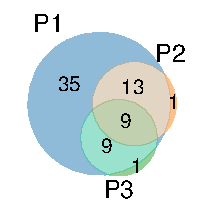
\includegraphics[width=0.5\textwidth]{countVenn.pdf}
		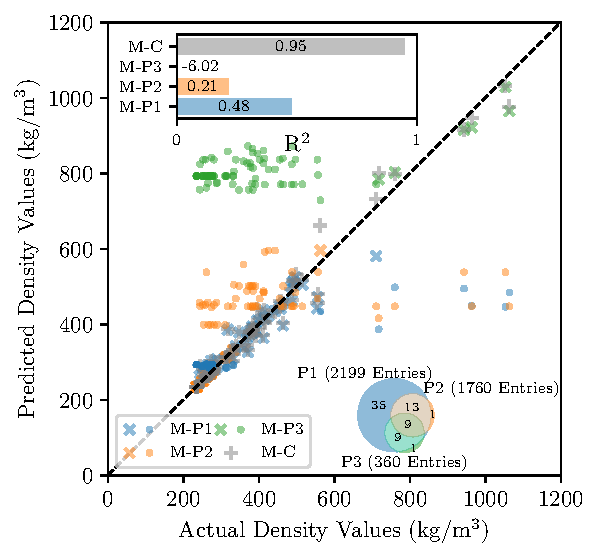
\includegraphics[width=0.5\textwidth]{scatterPlot.pdf}
		\caption{(Top-Left) Shows bar graph of number of entries obtained from each provider and the total number of entries.} 
	\end{figure}
	The OPTIMADE API enables a user to obtain material information from multiple databases with the same filter query. This is particularly useful when applying machine learning techniques on the obtained materials data. Being able to query multiple databases using a single API allows one to combine data from multiple sources, which may have different relative "strengths". As a demonstration of 
	
	OPTIMADE simplifies the workflow in many different machine learning applications. 
\end{document}